\chapter{Analysis of Results} % (fold)
\label{cha:analysis_of_results}

The experiments and their results show a number of things: the approach of exemplar-NBNN detection works not only on the TUD dataset, but also fairly well on the VOC 2007 set. Furthermore, the substitution of the agglomerative clustering algorithm with a mode finding algorithm seems to have a positive effect, just like taking a value of $k>1$ and using LNBNN. Nevertheless there is much variance within the results, and therefore it is necessary to give a deeper analysis of the results, to find out how they can be interpreted.

A first glance at the results might show which objects are relatively easy to detect, which ones are hard, and what images succeed in ``deceiving'' the LNBNN. Figure~\ref{fig:dettp} shows the four highest ranked ``True Positive'' detections of persons in the experiment with the best median AP for VOC 2007 (cf. Table~\ref{tab:vocallaps}). Strikingly, all objects are large, covering over half of the image. Compared to the highest ranked ``False Positives'' in Figure~\ref{fig:detfp}, it shows that all highly ranked detections cover all or most of the image. Figure~\ref{fig:bbsizevsrank} confirms this suspicion that highly ranked detections tend to be larger on average than the lower ranked ones. Taking into account the ranking method, which gives larger clusters a higher rank ($Q_D$), this means that the larger the cluster is, the more likely that the detections are large in image coverage.

\begin{figure}[hbt]
    \centering
    \begin{subfigure}[b]{0.45\textwidth}
        \centering
        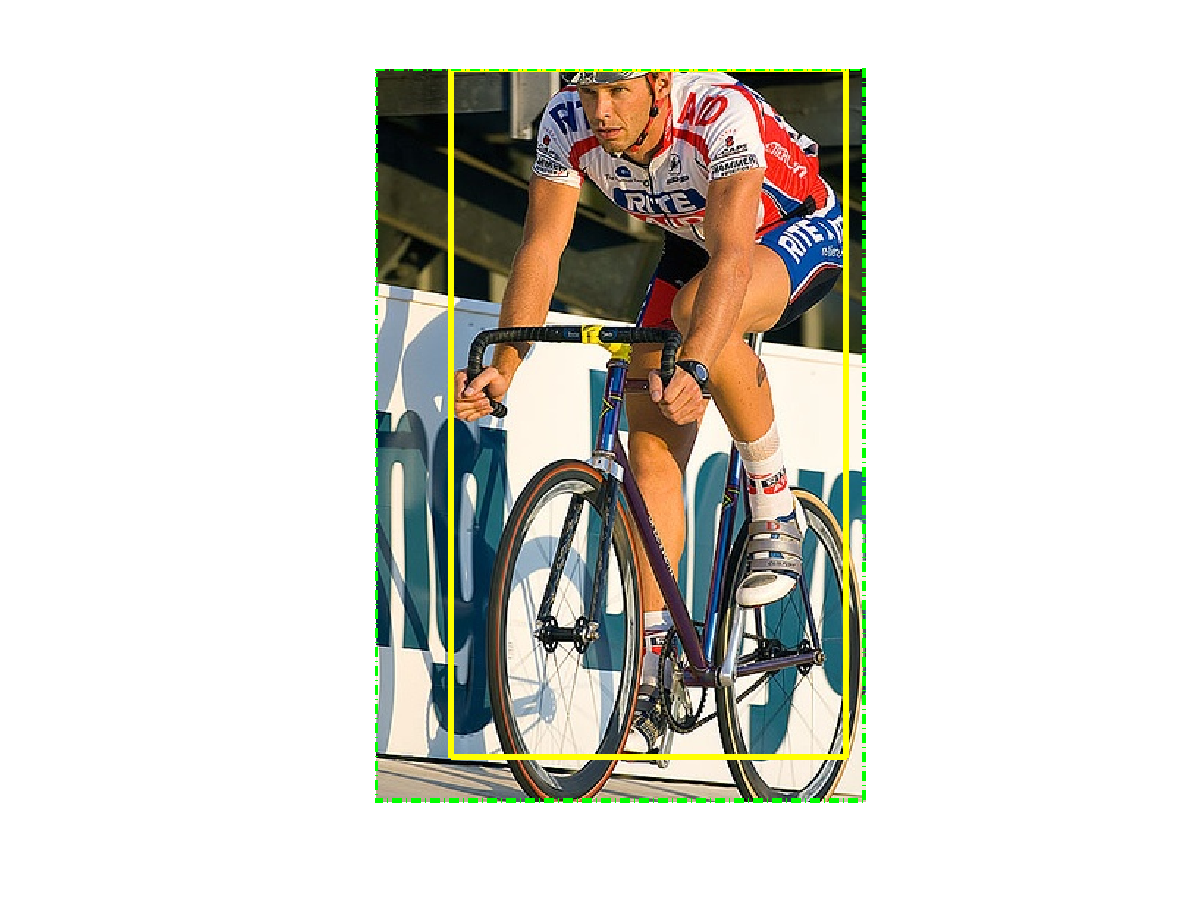
\includegraphics[width=\textwidth]{TP34}
        \caption{}
        \label{fig:dettp1}
    \end{subfigure}
    ~
    \begin{subfigure}[b]{0.45\textwidth}
        \centering
        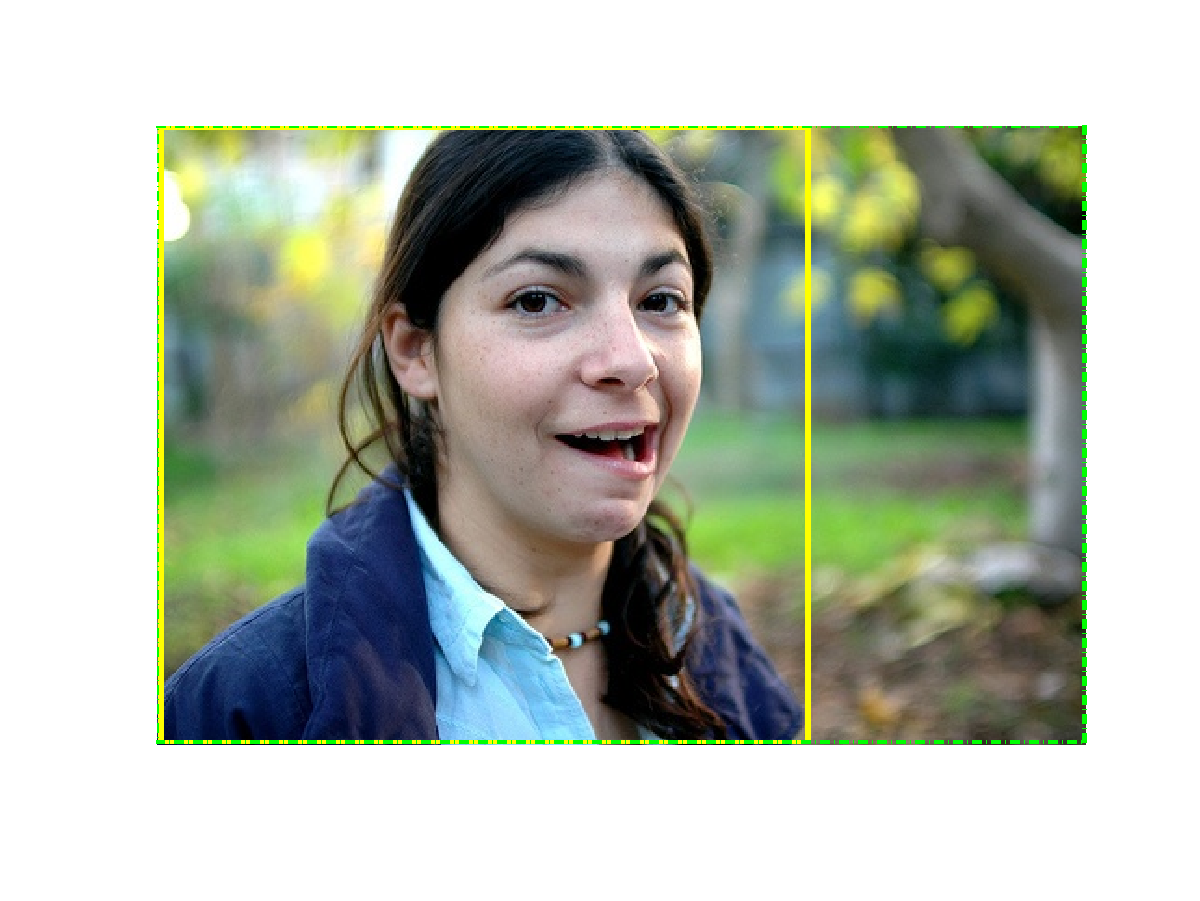
\includegraphics[width=\textwidth]{TP43}
        \caption{}
        \label{fig:dettp2}
    \end{subfigure}
    
    \begin{subfigure}[b]{0.45\textwidth}
        \centering
        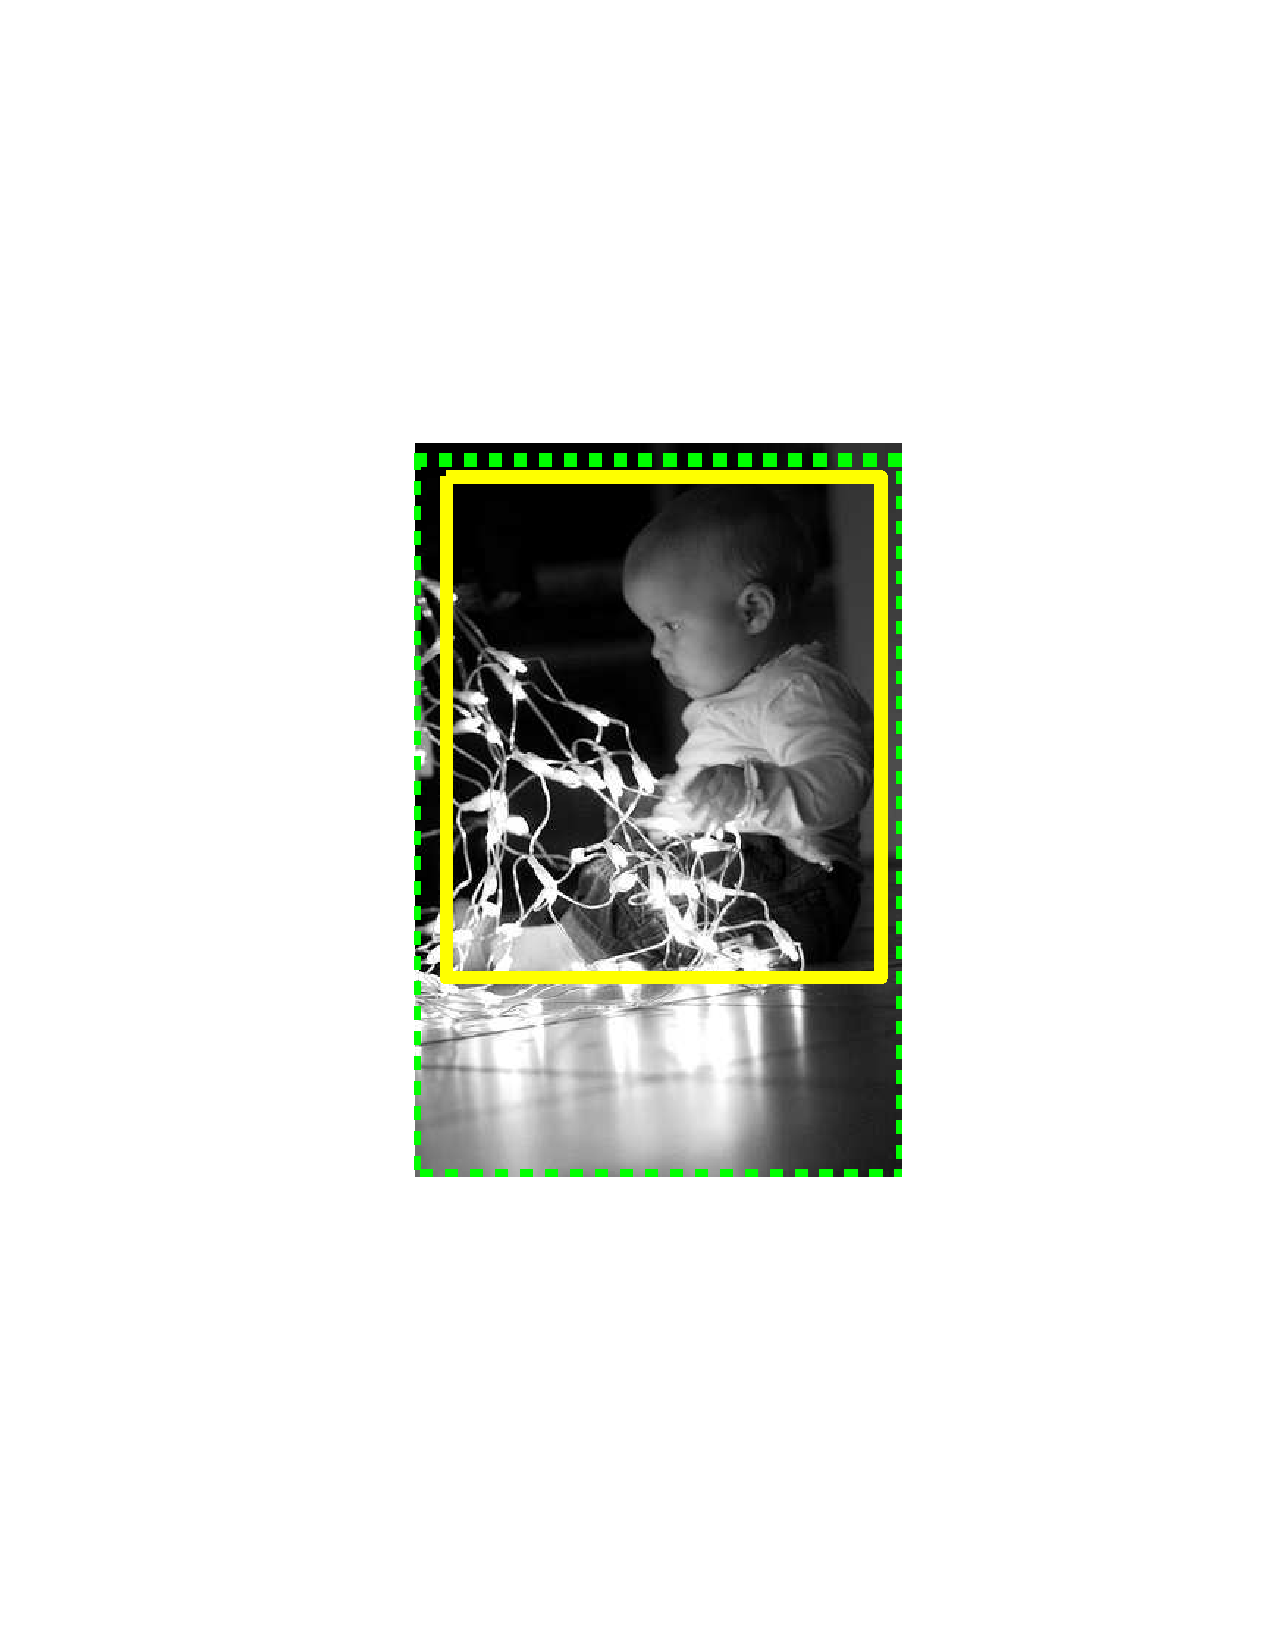
\includegraphics[width=\textwidth]{TP48}
        \caption{}
        \label{fig:dettp3}
    \end{subfigure}
    ~
    \begin{subfigure}[b]{0.45\textwidth}
        \centering
        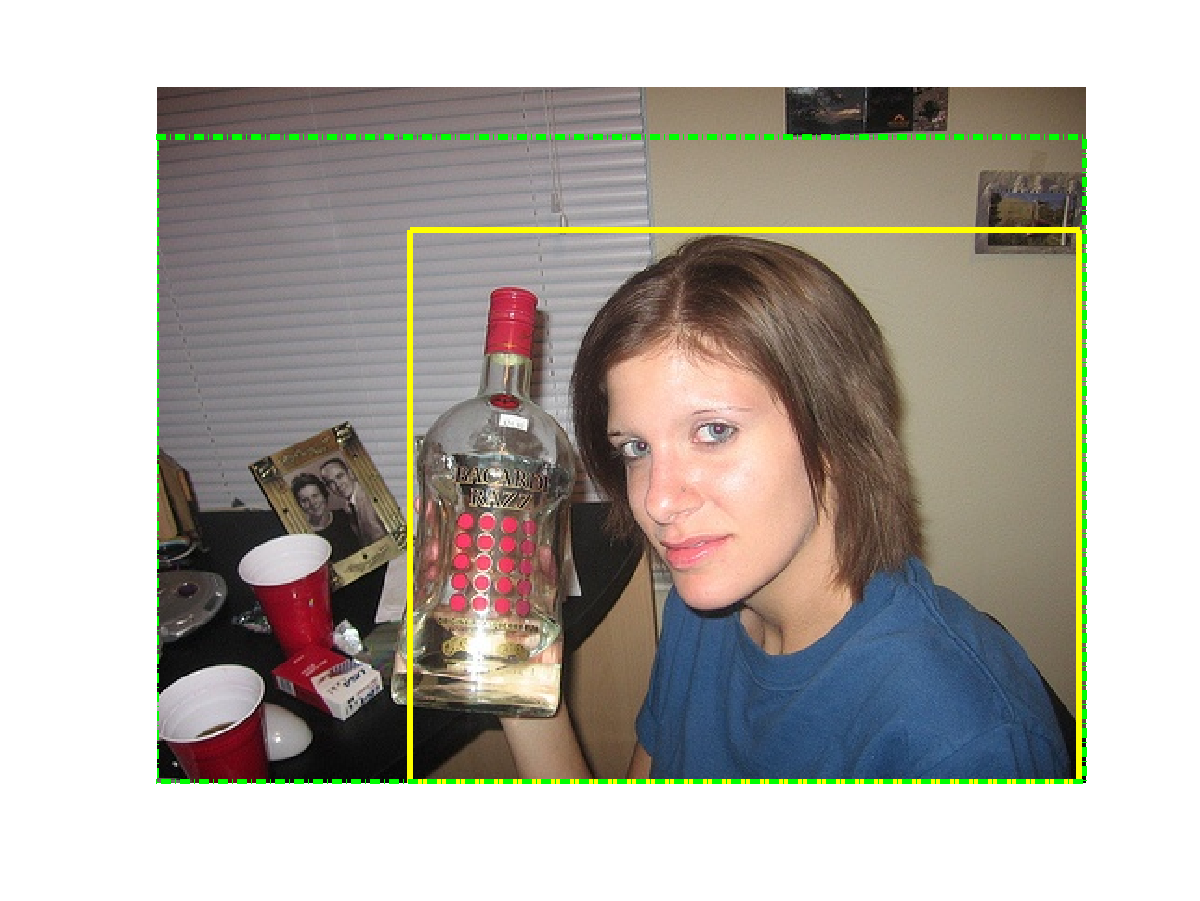
\includegraphics[width=\textwidth]{TP63}
        \caption{}
        \label{fig:dettp4}
    \end{subfigure}
    \caption{``True Positives'', correct detections with the highest rank, using LNBNN, $k=4$, interest point detection and quickshift ($\tau=1.2$) on the VOC 2007 person class.}
    \label{fig:dettp}
\end{figure}

Taking a closer look at Figure~\ref{fig:detfp}, it shows that besides a near miss of a person detection, the other false positives involve large objects, but of the wrong class.

On the other end of the detection ranking are hard-to-guess persons, that have nevertheless been detected. Note that because the recall is lower than 1, some persons have not been detected at all. The hard-to-guess persons shown in Figure~\ref{fig:dettn} are mostly small, occluded, or cut-off. besides, in some images large objects of other classes are pictured, which may have influenced the number of hypotheses for the person-class in these particular images.

\begin{figure}[hbt]
    \centering
    \begin{subfigure}[b]{0.45\textwidth}
        \centering
        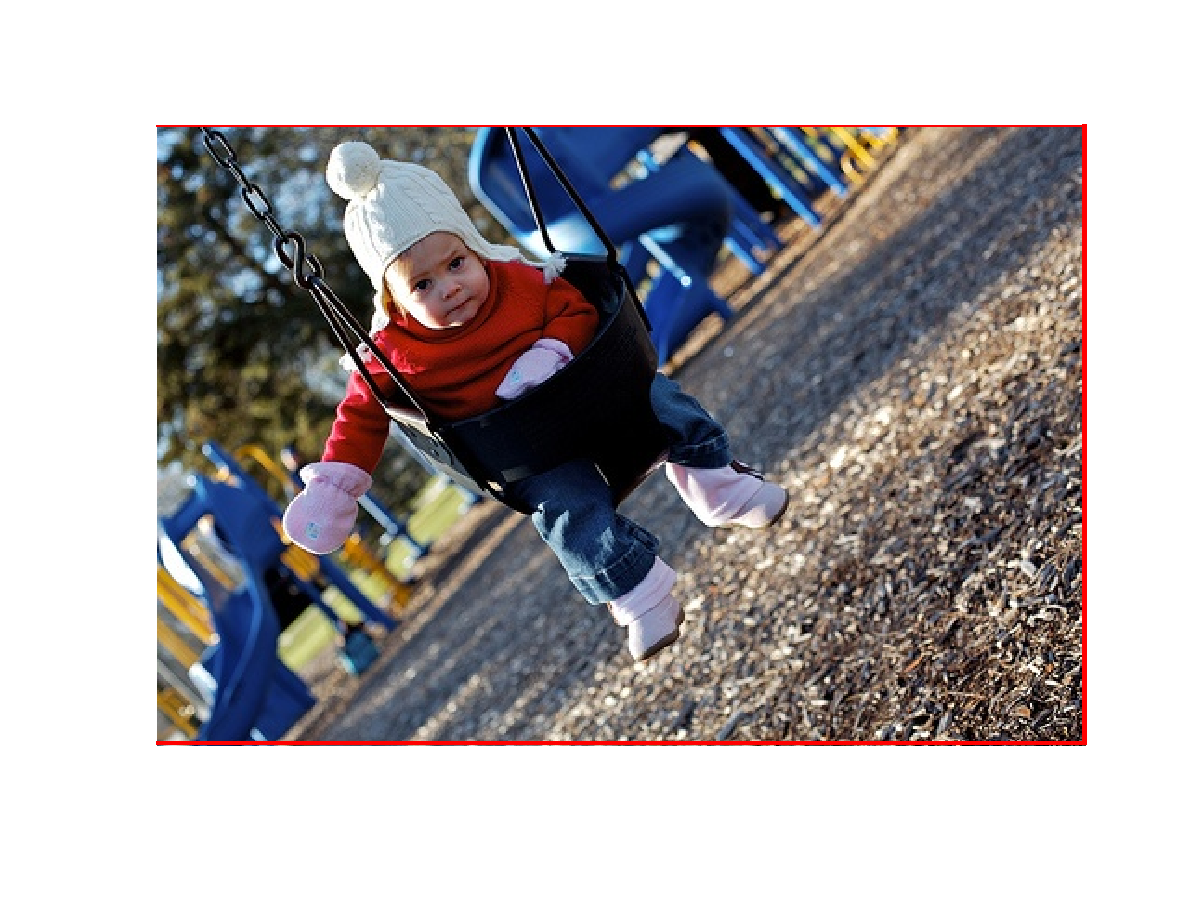
\includegraphics[width=\textwidth]{FP1}
        \caption{}
        \label{fig:detfp1}
    \end{subfigure}
    ~
    \begin{subfigure}[b]{0.45\textwidth}
        \centering
        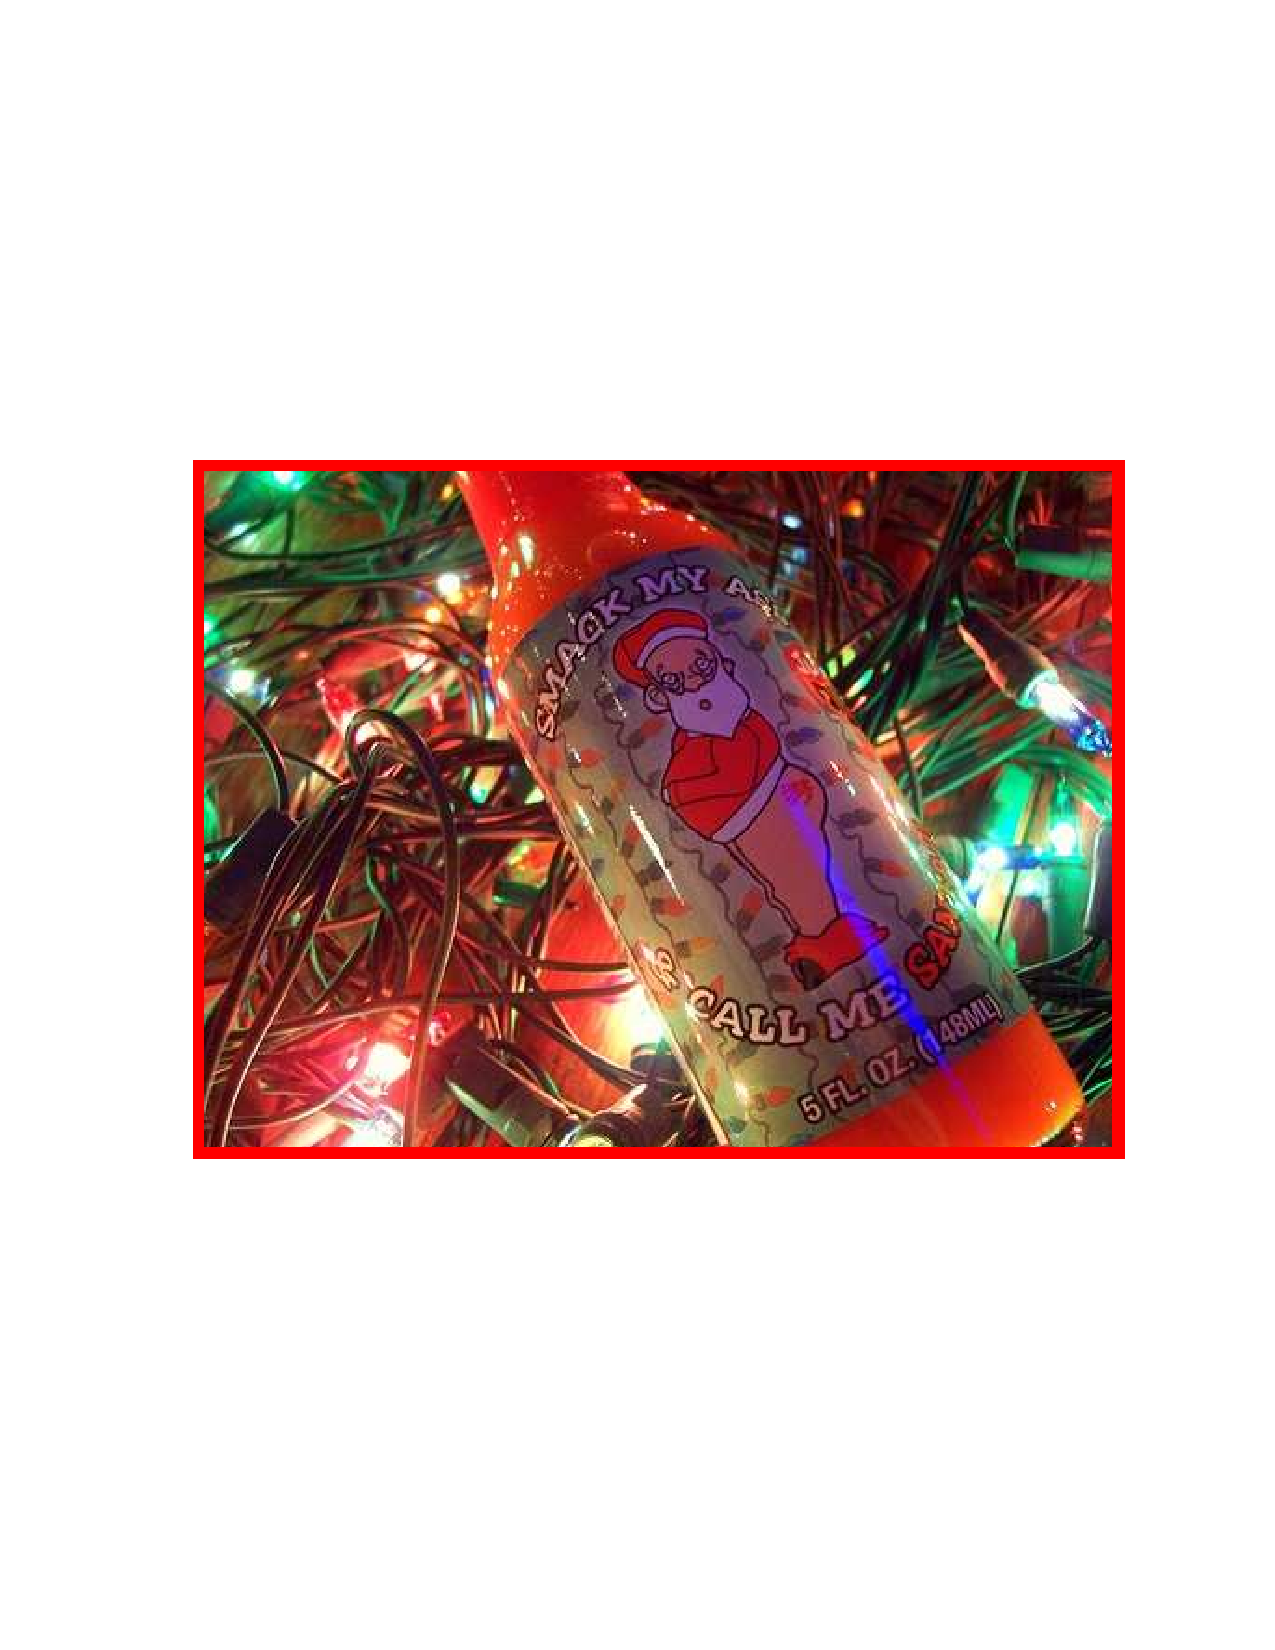
\includegraphics[width=\textwidth]{FP2}
        \caption{}
        \label{fig:detfp2}
    \end{subfigure}
    
    \begin{subfigure}[b]{0.45\textwidth}
        \centering
        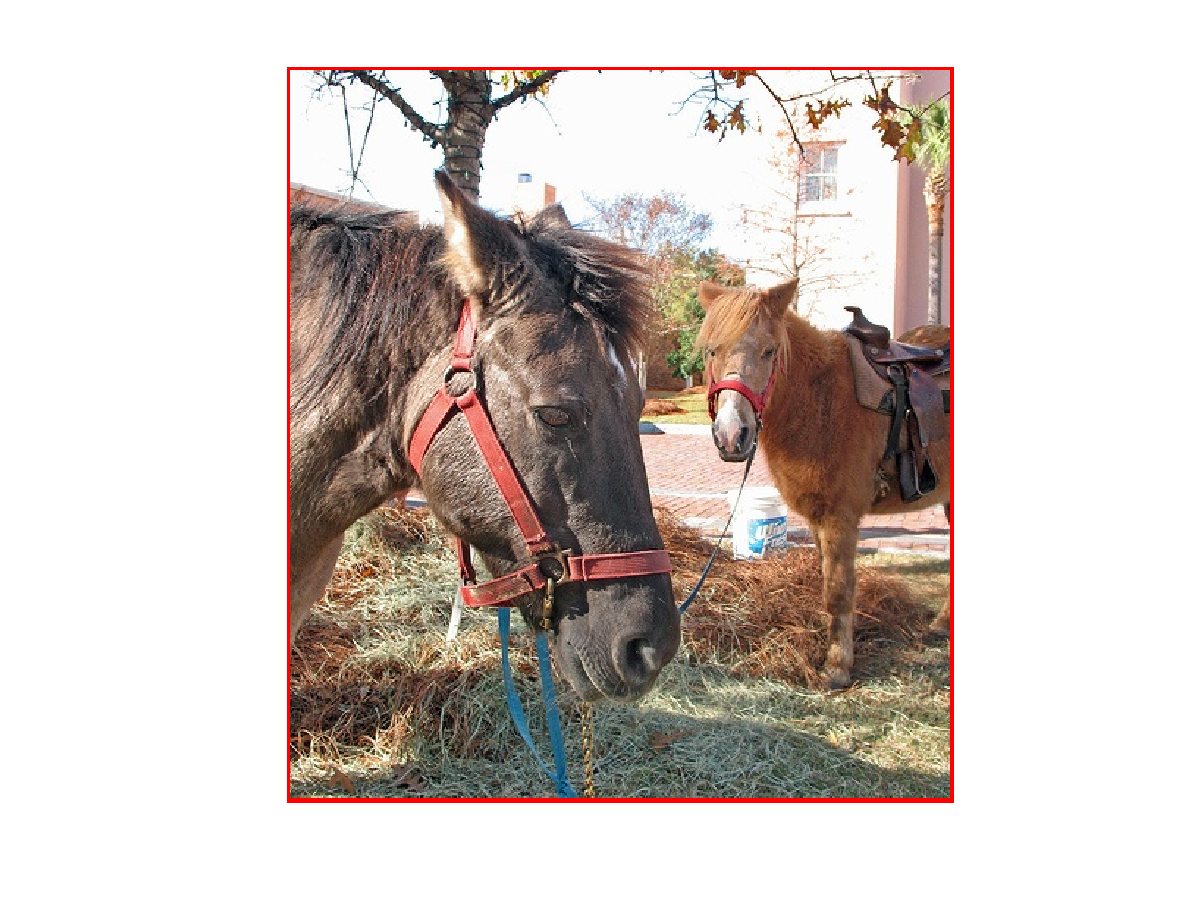
\includegraphics[width=\textwidth]{FP3}
        \caption{}
        \label{fig:detfp3}
    \end{subfigure}
    ~
    \begin{subfigure}[b]{0.45\textwidth}
        \centering
        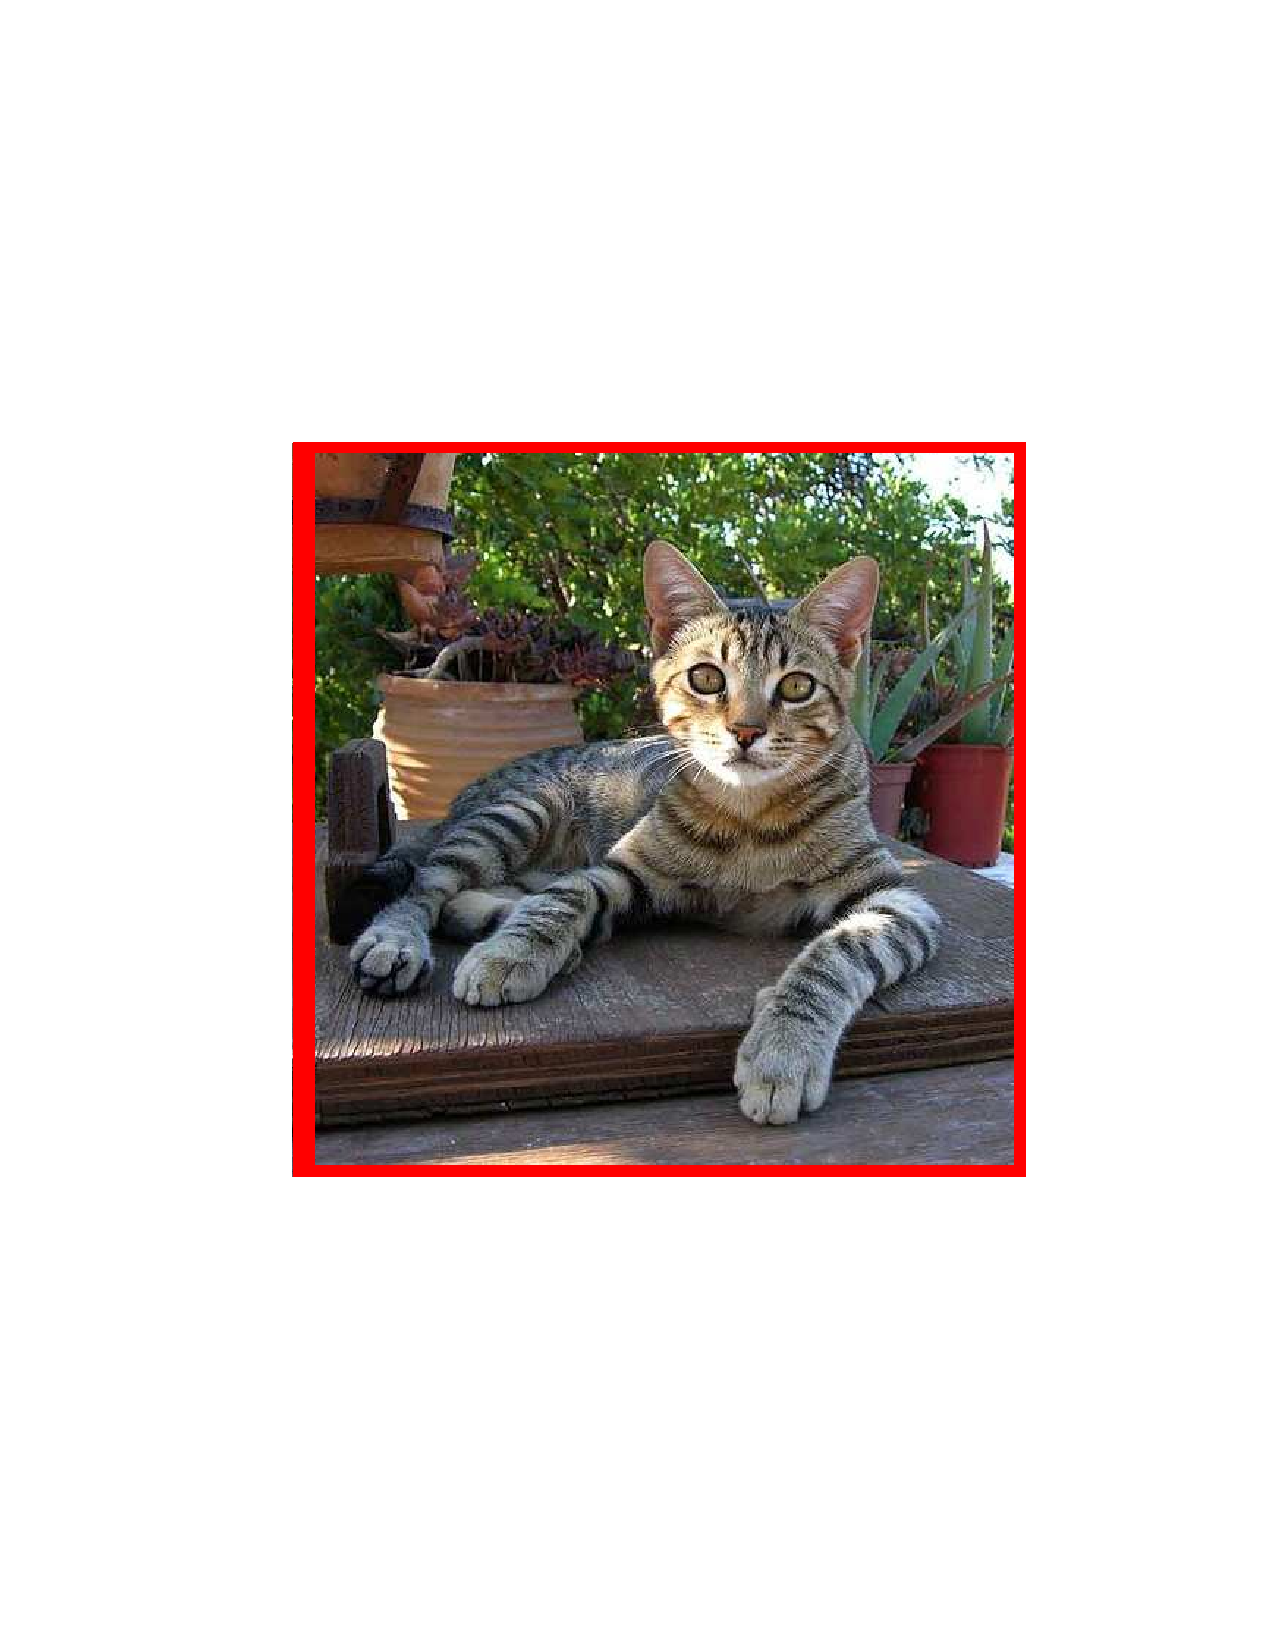
\includegraphics[width=\textwidth]{FP4}
        \caption{}
        \label{fig:detfp4}
    \end{subfigure}
    \caption{``False Positives'', incorrect detections with the highest rank, using LNBNN, $k=4$, interest point detection and quickshift ($\tau=1.2$) on the VOC 2007 person class. Note that all bounding boxes envelop the whole image.}
    \label{fig:detfp}
\end{figure}

\begin{figure}[hbt]
    \centering
    \begin{subfigure}[b]{0.45\textwidth}
        \centering
        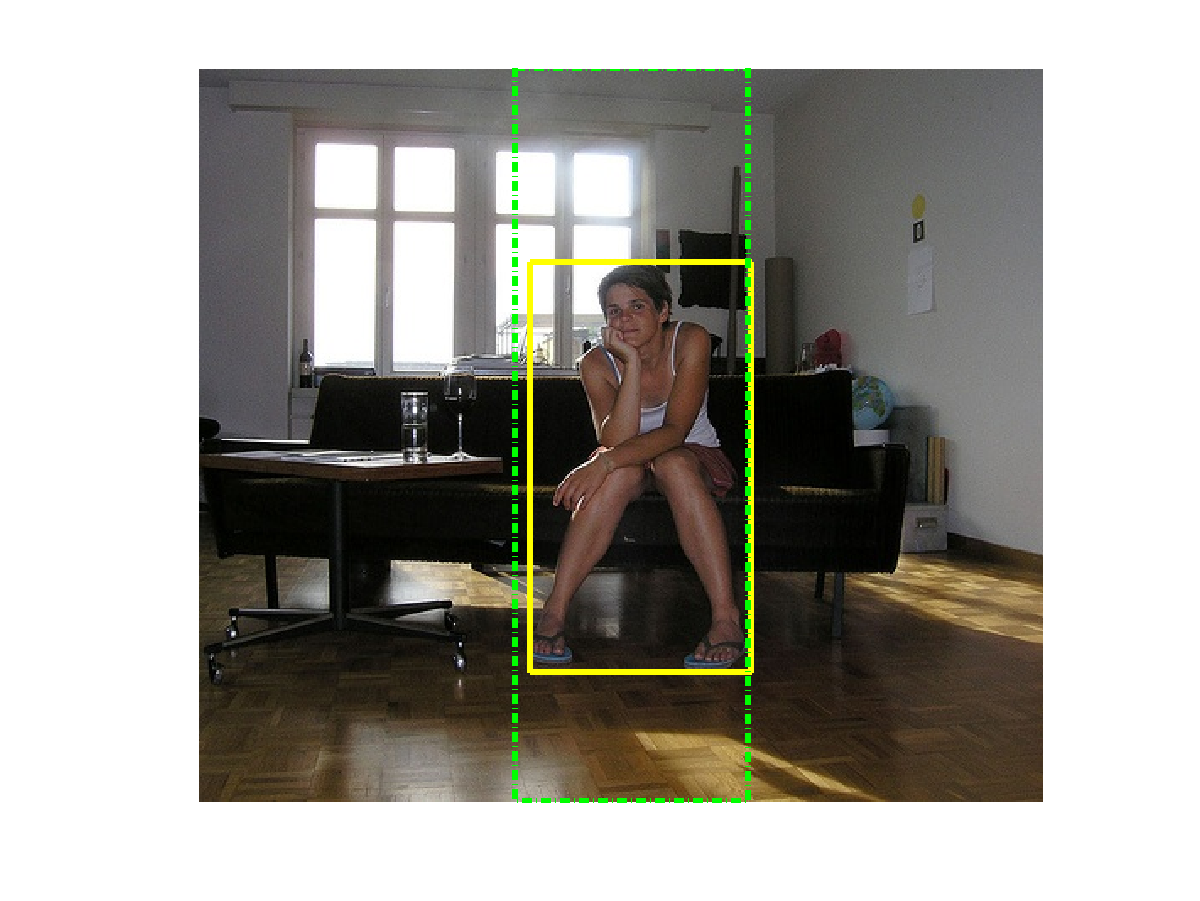
\includegraphics[width=\textwidth]{TP31116}
        \caption{}
        \label{fig:dettn1}
    \end{subfigure}
    ~
    \begin{subfigure}[b]{0.45\textwidth}
        \centering
        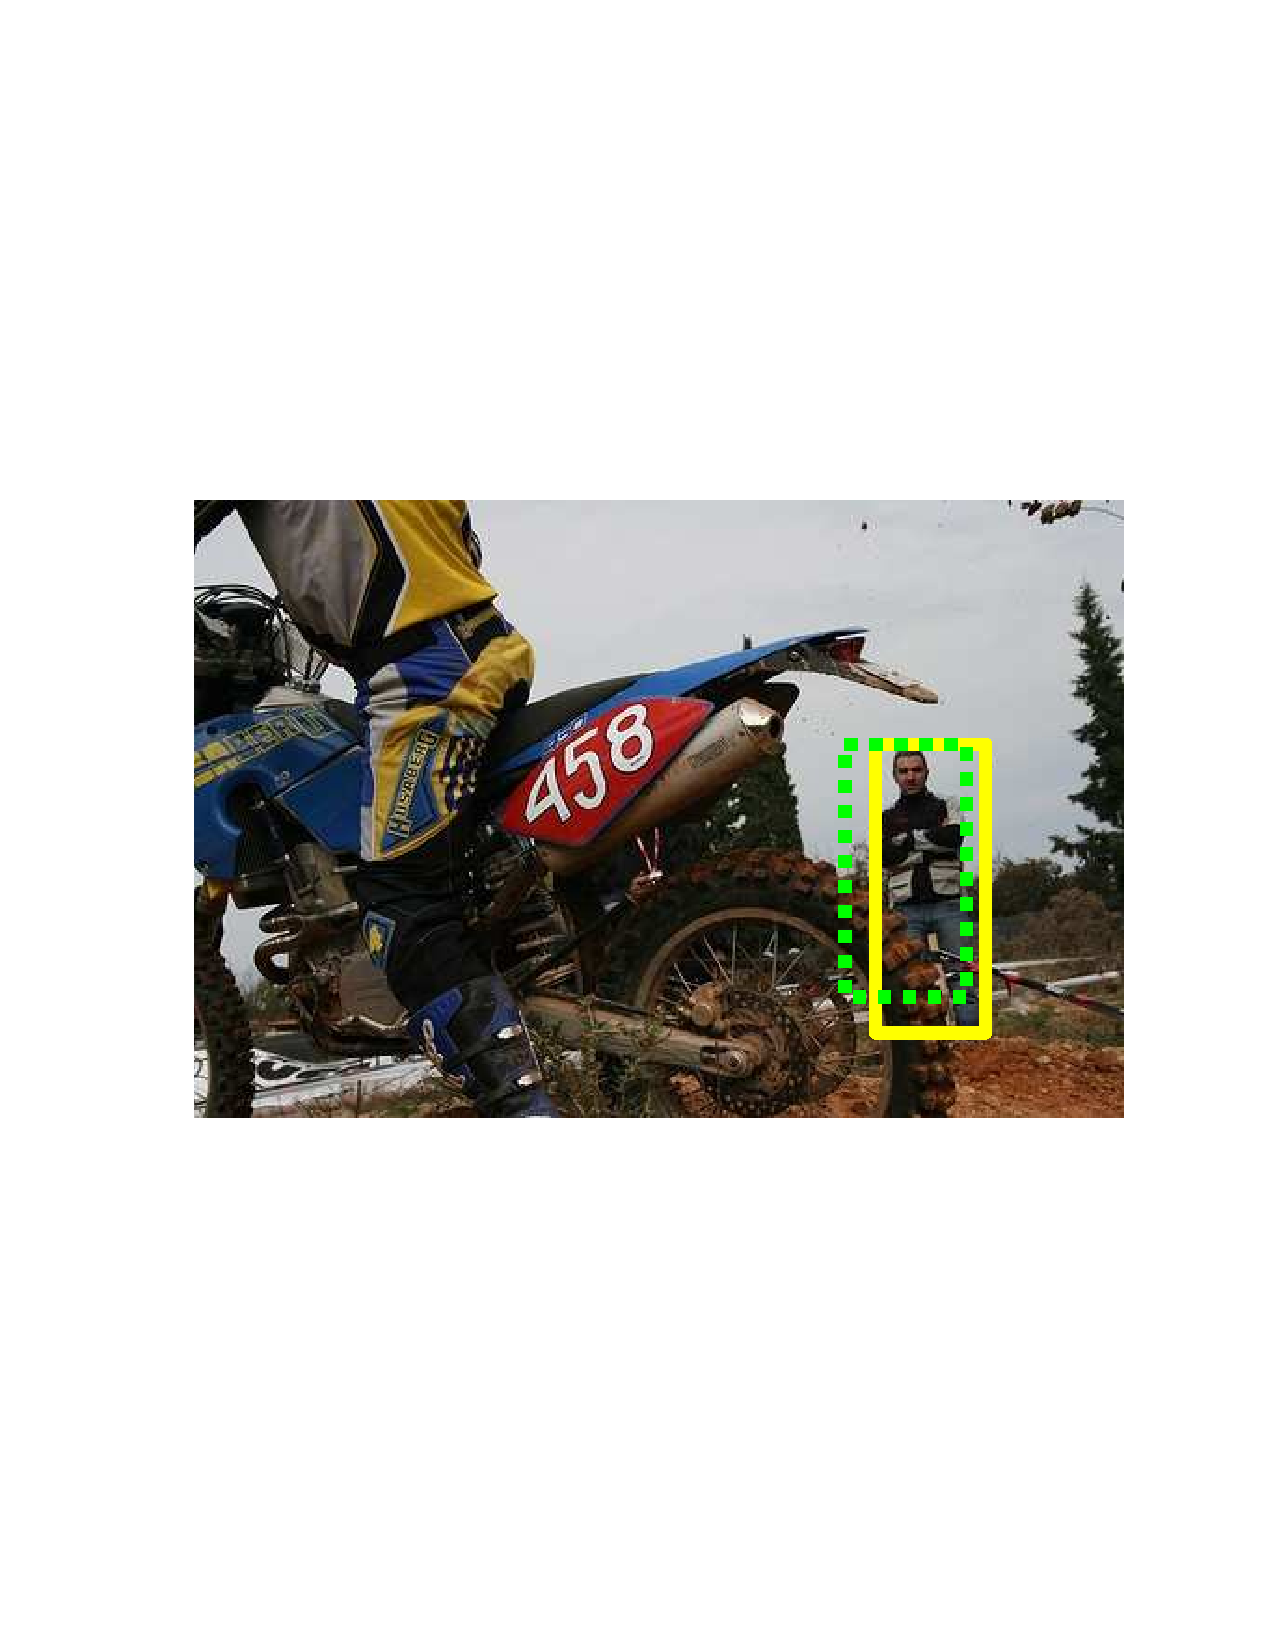
\includegraphics[width=\textwidth]{TP30971}
        \caption{}
        \label{fig:dettn2}
    \end{subfigure}
    
    \begin{subfigure}[b]{0.45\textwidth}
        \centering
        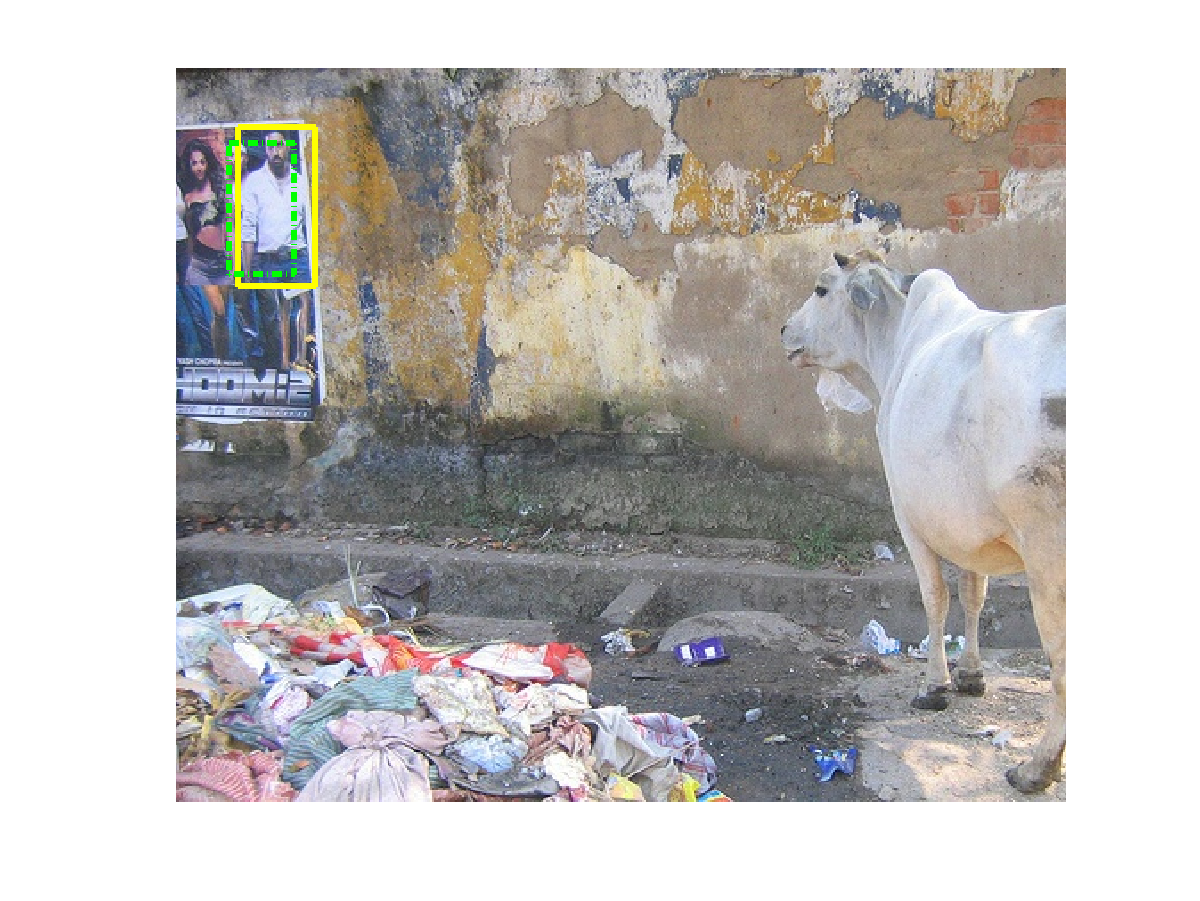
\includegraphics[width=\textwidth]{TP30932}
        \caption{}
        \label{fig:dettn3}
    \end{subfigure}
    ~
    \begin{subfigure}[b]{0.45\textwidth}
        \centering
        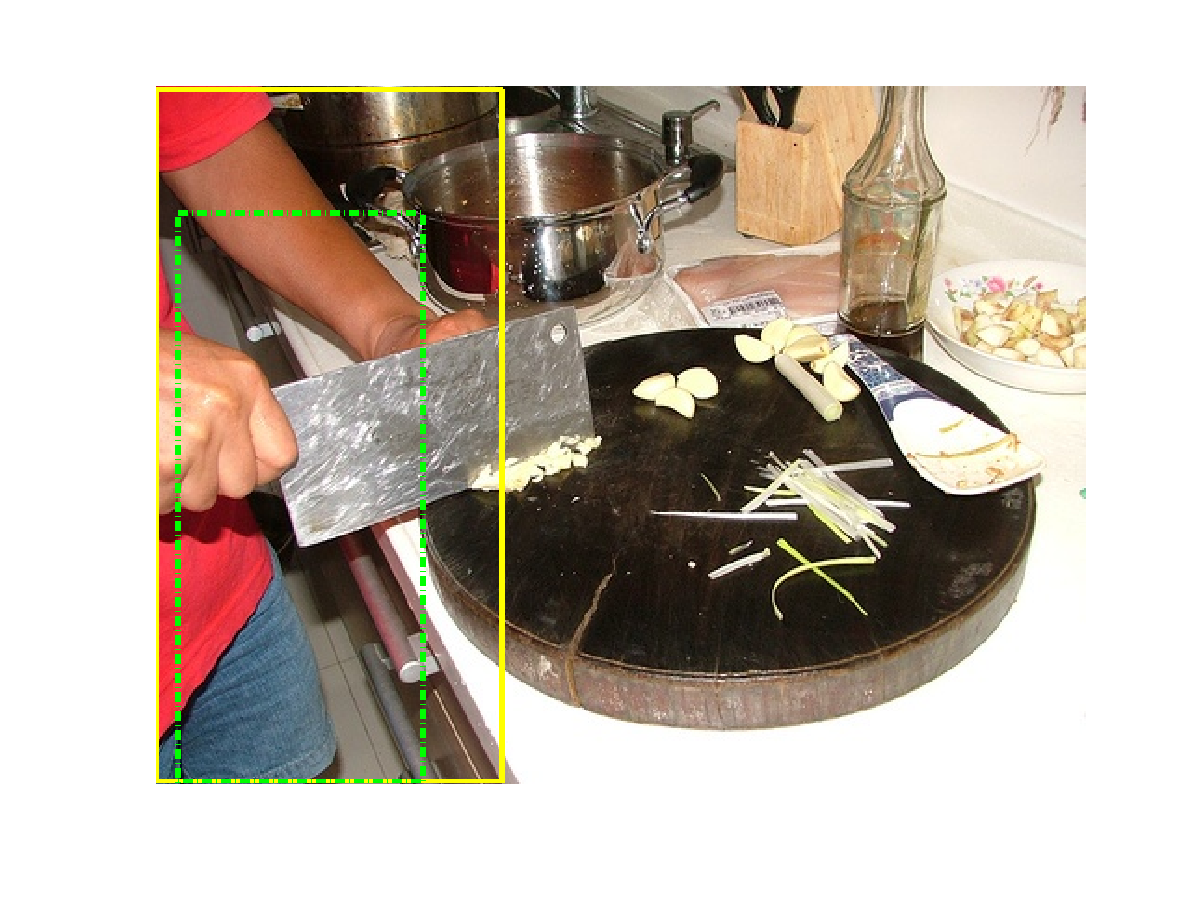
\includegraphics[width=\textwidth]{TP30705}
        \caption{}
        \label{fig:dettn4}
    \end{subfigure}
    \caption{``Difficult'', correct detections with the lowest ranks, using LNBNN, $k=4$, interest point detection and quickshift ($\tau=1.2$) on the VOC 2007 person class.}
    \label{fig:dettn}
\end{figure}

\begin{figure}[hbt]
    \centering
    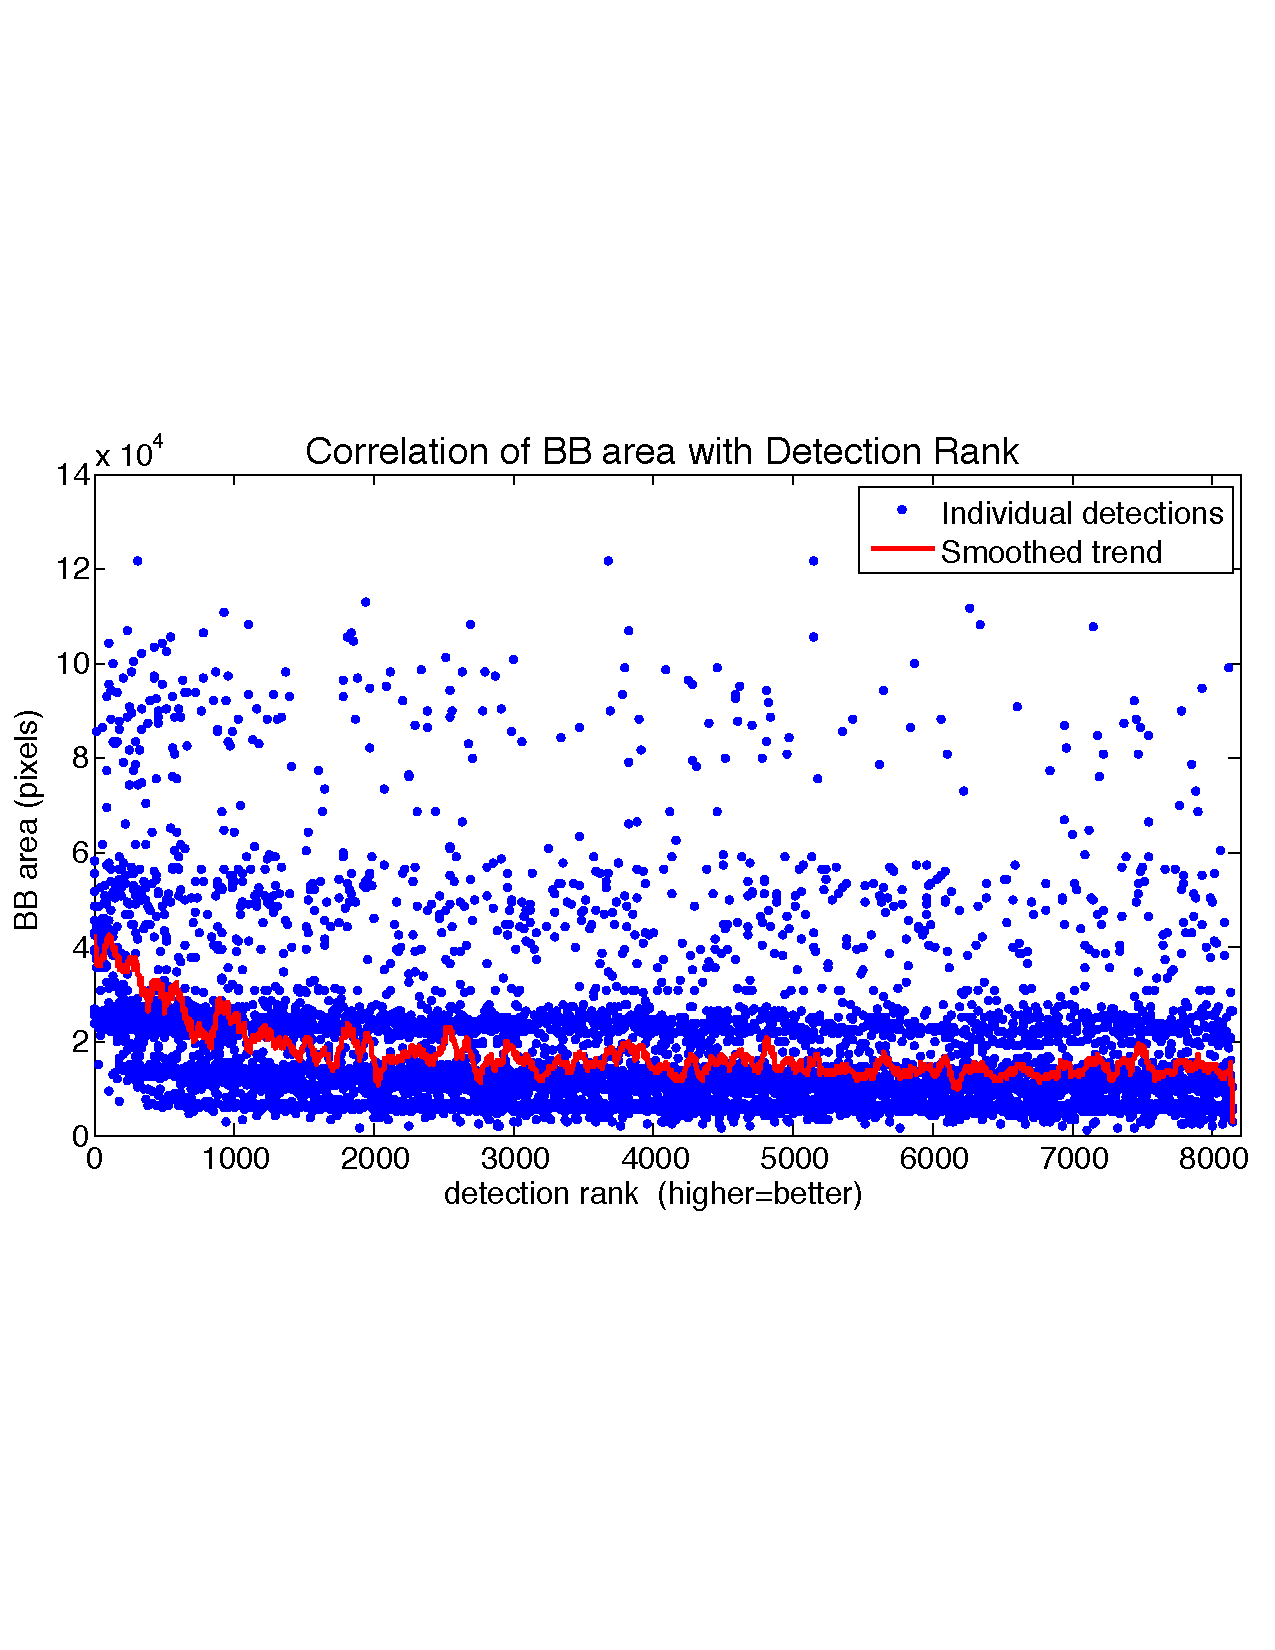
\includegraphics[width=0.9\textwidth]{BBSizeVsRank}
    \caption{The experiments show that the detections with a higher rank (from a larger cluster), also have a tendency to generate larger bounding boxes. This graph comes from the TUD motorbike experiment using $k=4$, quickshift ($\tau=1.2$) and dense sampling.}
    \label{fig:bbsizevsrank}
\end{figure}

In the next sections certain aspects of the experiments are analyzed in more depth.

\section{The Datasets} % (fold)
\label{sec:the_dataset}

The differences between the datasets are striking. The TUD Motorbikes set has a single class, and the test set contains only positive images (i.e. images with at least one motorbike). The training set has a clear-cut segmentation, which improves the feature quality. The VOC 2007 dataset is much harder. Every class appears in only 5\% of the test images, excluding the \emph{person} class, which occurs in 40\% of the images. To put it another way, in the TUD Motorbike test the task is for every image to locate the motorbike object(s), while in de VOC 2007 test the task is for every image and every class to assess the possibility of this class having an object in the image, and if yes, to locate it.

Of course, in practice these tasks are modeled in the same way. The detections within a single class are all compared to one another in terms of their value (cluster size), across all images, both class and non-class images (\emph{cf.} the PASCAL VOC evaluation method \cite{pascal-voc-2007}).

Another important aspect is that the TUD dataset tends to have motorbike objects that are large, centered in the image, and with little clipping and occlusion. Some of the classes of VOC 2007 consist of objects that are generally small (\emph{bottle}), not in the focal point of the image (\emph{chair, pottedplant}), or often occluded by other objects (\emph{diningtable}). This makes it obvious that the scores overall are higher on the TUD Motorbikes test than on the VOC 2007 test.
% It raises the question however whether exemplar-NBNN might perform relatively better, or worse, on the TUD motorbikes test than on the VOC 2007 set.
% It is difficult to compare this to other methods, because the TUD set is not regularly used in the literature. It is possible however to visualize what kinds of objects in both tests are hard to detect, and which ones are easy. This might give more insight in the mechanics of the algorithm.


% subsection the_dataset (end)

\section{Clustering Algorithms} % (fold)
\label{sub:anal_clustering_algorithms}

Overall, the suspicion seems to be correct that quickshift should perform better than agglomerative clustering because of the more natural way of selecting a cluster center, i.e. a detection out of a cluster of hypotheses. The results however depend a lot on class, and are not always very obvious.

To see whether the clustering of hypotheses is needed at all, for some tests a comparison was made between the performance of the ranked detections versus ranking the hypotheses. As a ranking method, Becker's $Q_H$ measure was used (Equation~\ref{eq:qh}). Figure~\ref{fig:hyprank} shows the effects of clustering on a small test.

\begin{figure}[hbt]
    \centering
    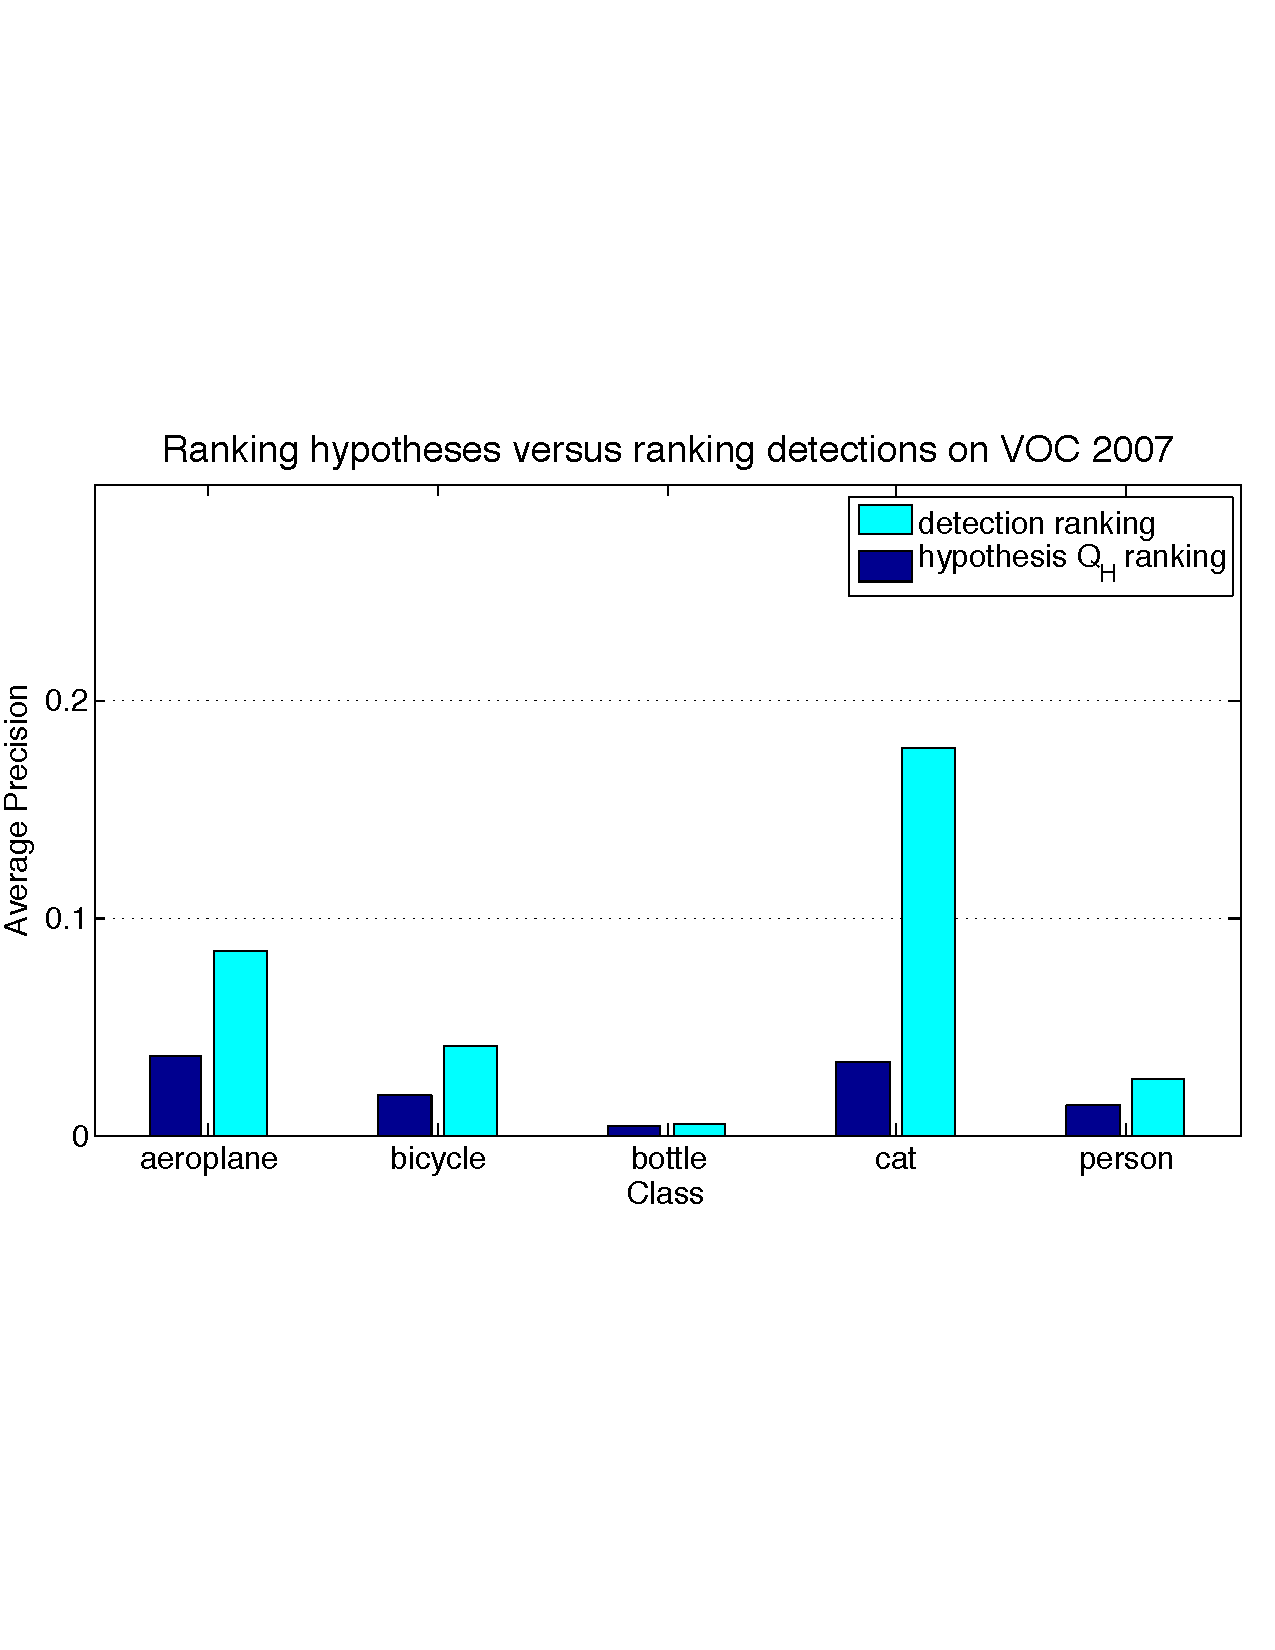
\includegraphics[width=0.9\textwidth]{APcomparehypdet}
    \caption{Comparison of Average Precision using the clustered detections versus the hypotheses before clustering, for a small test on 5 VOC 2007 classes, using LNBNN with $k=5$, quickshift clustering, and interest point detection. It clearly shows the effect of clustering.}
    \label{fig:hyprank}
\end{figure}

The recall of the detections will usually be lower than the recall when using hypotheses, because the detections are more or less a subset of hypotheses. However, ranking the hypotheses appears to be much harder than ranking detections, resulting in a much lower AP. This shows the main benefit of clustering.

% subsection clustering_algorithms (end)

\section{The Influence of $k$} % (fold)
\label{sub:the_influence_of_k_}

The experiments show that performance increases when multiple neighbors are taken into account, confirming the theory of descriptor aliasing in Section \ref{sec:descriptor_aliasing}. There is however a quite narrow sweet spot: setting $k$ too high hurts performance and, to a larger extend, efficiency. On the TUD set, with only two classes (motorbike and background), the ideal value for $k$ will be lower than on the VOC 2007 set, having 21 classes. As McCann \& Lowe \cite{mccann2012local} show, $k$ should be a multiple of the number of classes to give a good estimate of the feature's local surroundings, and of the classes which are relatively close to it. With $k$ as low as 5, at most 5 classes can be included as nearest neighbors, which might not give a fair estimate for the other classes.

Unfortunately, setting $k$ higher has been proven prohibitive when running quickshift tests on the VOC 2007 set. A more efficient algorithm could explore the influence of $k$ much better.

% subsection the_influence_of_k_ (end)

\section{Time and Memory} % (fold)
\label{sub:time_and_memory_constraints}

Detection algorithms can be compared not only for their qualitative performance, but also in terms of complexity and efficiency. Exemplar-NBNN is quite heavy in both terms. Given $t$ training images, $s$ test images, $d$ descriptors per image, on average, $c$ classes, and $k$ nearest neighbors, this is the time complexity breakdown of the main stages of the pipeline:
\begin{enumerate}
    \item Extracting features from the training images, splitting them into the classes, adding them to their respective NN indexes and saving their exemplars: $\frac{td}{c} \log \frac{td}{c} = O(n\log n)$, using FLANN kd-trees for building NN indexes.
    \item Extracting features from the test images: $s\times d$
    \item Finding $k$ nearest neighbors from each class, for each descriptor of each test image: $d s c \log \frac{td}{c} = O(n \log n)$, using kd-trees.
    \item Performing detection. For each test image and each class, get its hypotheses, calculated their pairwise overlap, and cluster them: $s c x (d k)^2 = O(n^2)$, factor $x>1$ depending on the clustering algorithm, but at least once for the pairwise overlap.
\end{enumerate}

\begin{figure}[hbt]
    \centering
    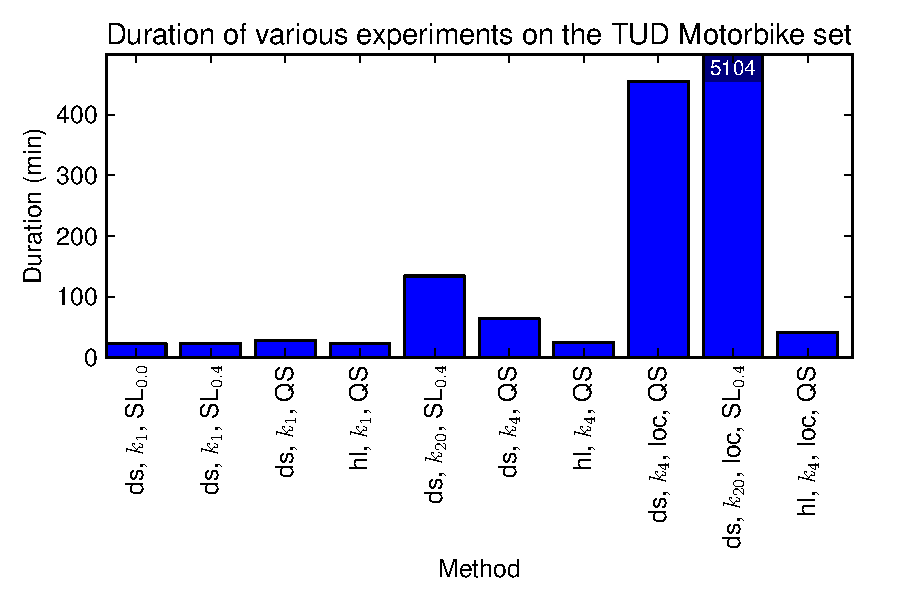
\includegraphics[width=0.9\textwidth]{DurTUD}
    \caption{Obviously duration increases as the experiments get more complex. LNBNN takes much more time, while the use of interest points causes a significant time reduction on tests with $k>1$.}
    \label{fig:durationTUD}
\end{figure}

\begin{figure}[hbt]
    \centering
    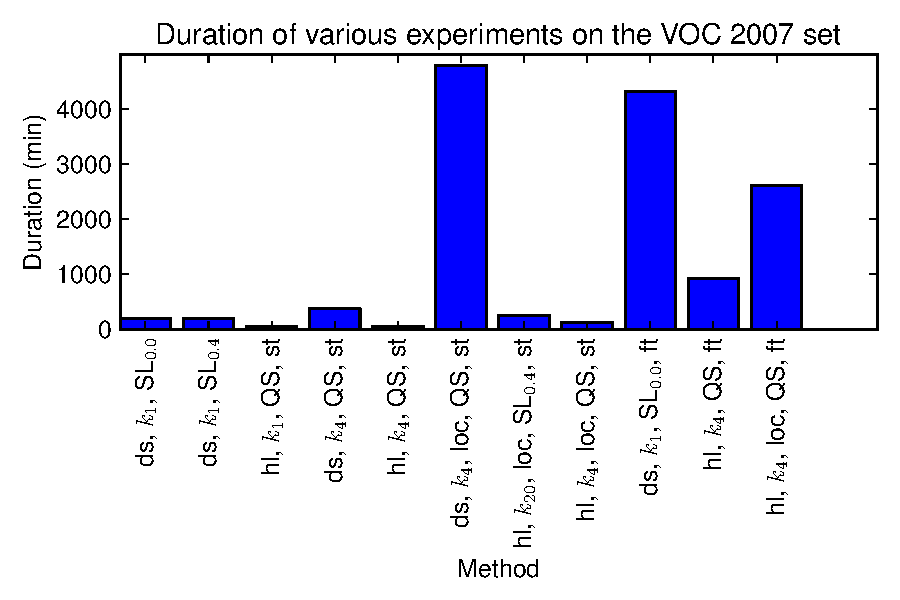
\includegraphics[width=0.9\textwidth]{DurVOC}
    \caption{The same trend is visible when testing on the VOC 2007 set. Especially the combination of dense sampling and Local NBNN is prohibitive. The three rightmost columns show tests run on the full VOC test set ($\sim$ 5000 images), whereas the other experiments were run on the segmentation test set of 210 images}
    \label{fig:durationVOC}
\end{figure}

This shows that the training phase has complexity $O(n\log n)$, while the test phase has complexity $O(n^2)$. This means training is quite efficient, mainly because no learning is involved. Testing takes much more time however, and proves to be the prohibitive step, especially calculating pairwise distances between all hypotheses in an image, for every image. Figure~\ref{fig:durationTUD} and~\ref{fig:durationVOC} show the duration of the experiments discussed in the previous section. The combination of LNBNN and dense sampling seems to increase duration greatly. Dense sampling results in a much larger value $d$ per image, causing both training and testing to take more time, especially the factor $(dk)^2$ during the detection phase, because $d\gg k$. LNBNN also takes into account more NN than plain $k$NBNN, but should not have this great an effect.

Increasing time complexity is somewhat correlated to memory complexity, especially in the biggest factor involved, the number of descriptors per image $d$. Both the FLANN indexes and the test image representations get bigger. This effect may cause additional issues when the experiment runs out of memory (memory swapping). This is probably the cause of the extremely large durations reported in Figures~\ref{fig:durationTUD} and~\ref{fig:durationVOC}.

% subsection time_and_memory_constraints (end)


% section analysis_of_results (end)